\begin{figure}[H]
	\begin{center}
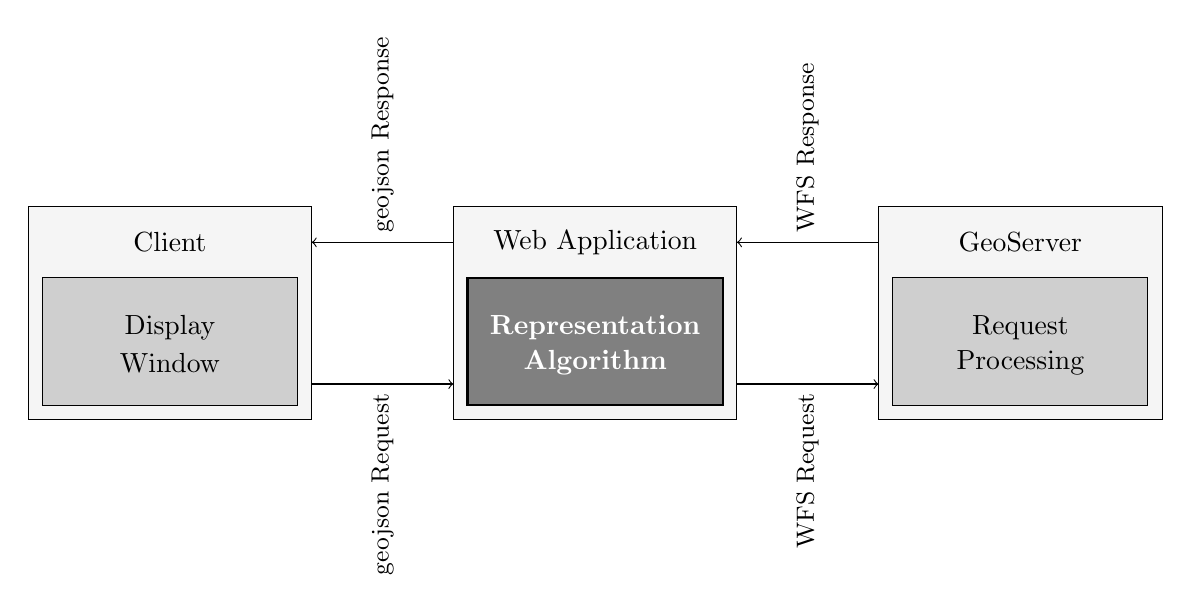
\begin{tikzpicture}[scale=0.9]
	\begin{scope}[]
		\fill[lightgray!15,draw=black] (0,0) rectangle (4,3);
		\fill[lightgray!75,draw=black] (0.2,0.2) rectangle (3.8,2);
		\node at (2,2.5) {Client};
		\node at (2,1.3) {Display};
		\node at (2,0.8) {Window};
	\end{scope}
	\begin{scope}[shift={(6,0)}]
		\fill[lightgray!15,draw=black] (0,0) rectangle (4,3);
		\fill[black!50,draw=black,thick] (0.2,0.2) rectangle (3.8,2);
		\node at (2,2.5) {Web Application};
		\node[text=white] at (2,1.3) {\textbf{Representation}};
		\node[text=white] at (2,0.8) {\textbf{Algorithm}};
	\end{scope}
	\begin{scope}[shift={(12,0)}]
		\fill[lightgray!15,draw=black] (0,0) rectangle (4,3);
		\fill[lightgray!75,draw=black] (0.2,0.2) rectangle (3.8,2);
		\node at (2,1.3) {Request};
		\node at (2,0.8) {Processing};
		\node at (2,2.5) {GeoServer};
	\end{scope}
	
	\begin{scope}[shift={(6,-0.5)},rotate=90]
		\draw[->] (1,2) -- node[left,rotate=90] {\small geojson Request} (1,0) ;
		\draw[<-] (3,2) -- node[right,rotate=90] {\small geojson Response} (3,0);
	\end{scope}


	\begin{scope}[shift={(12,-0.5)},rotate=90]
		\draw[->] (1,2) -- node[left,rotate=90] {\small WFS Request} (1,0) ;
		\draw[<-] (3,2) -- node[right,rotate=90] {\small WFS Response} (3,0);
	\end{scope}
\end{tikzpicture}
\end{center}
\caption{Proposed Program Architecture}
\label{fig:arch}
\end{figure}